\documentclass{article}
\usepackage[utf8]{inputenc}
\usepackage[english]{babel}
\usepackage{graphicx}
\usepackage{amsthm}

\DeclareGraphicsExtensions{.pdf,.ps,.png,.jpg}

\newcounter{results}

\newtheorem{theorem}{Theorem}[section]
\newtheorem{lemma}[theorem]{Lemma}
\newtheorem{corollary}{Corollary}[theorem]

\author{
  McCaffrey, Caitie\\
  \texttt{Sporty Tights, Inc}
  \and
  Kingsbury, Kyle\\
  \texttt{The SF Eagle}
  \and
  Narula, Neha\\
  \texttt{That's DOCTOR Narula to you!}
}

\title{Distributed Sagas}

\begin{document}

\maketitle

\section{Introduction}

The saga paper outlines a technique for long-lived transactions which provide
atomicity and durability without isolation (what about consistency? Preserved
outside saga scope, not within, right?). In this work, we generalize sagas to
a distributed system, where processes communicate via an asynchronous network,
and discover new constraints on saga sub-transactions.

We are especially interested in the problem of writing sagas which interact with
\textit{third-party services}, where we control the Saga Execution Coordinator
(SEC) and its storage, but not the downstream Transaction Execution
Coordinators (TECs) themselves. Communication between the SEC and TEC(s) takes
place over an asynchronous network (e.g. TCP) which is allowed to drop, delay,
or reorder messages, but not to duplicate them.

We assume a high-availability SEC service running on multiple nodes for
fault-tolerance, where multiple SECs may run concurrently. They coordinate
their actions through a linearizable data store, which ensures saga
transactions proceed sequentially.

\section{The Saga Execution Coordinator}

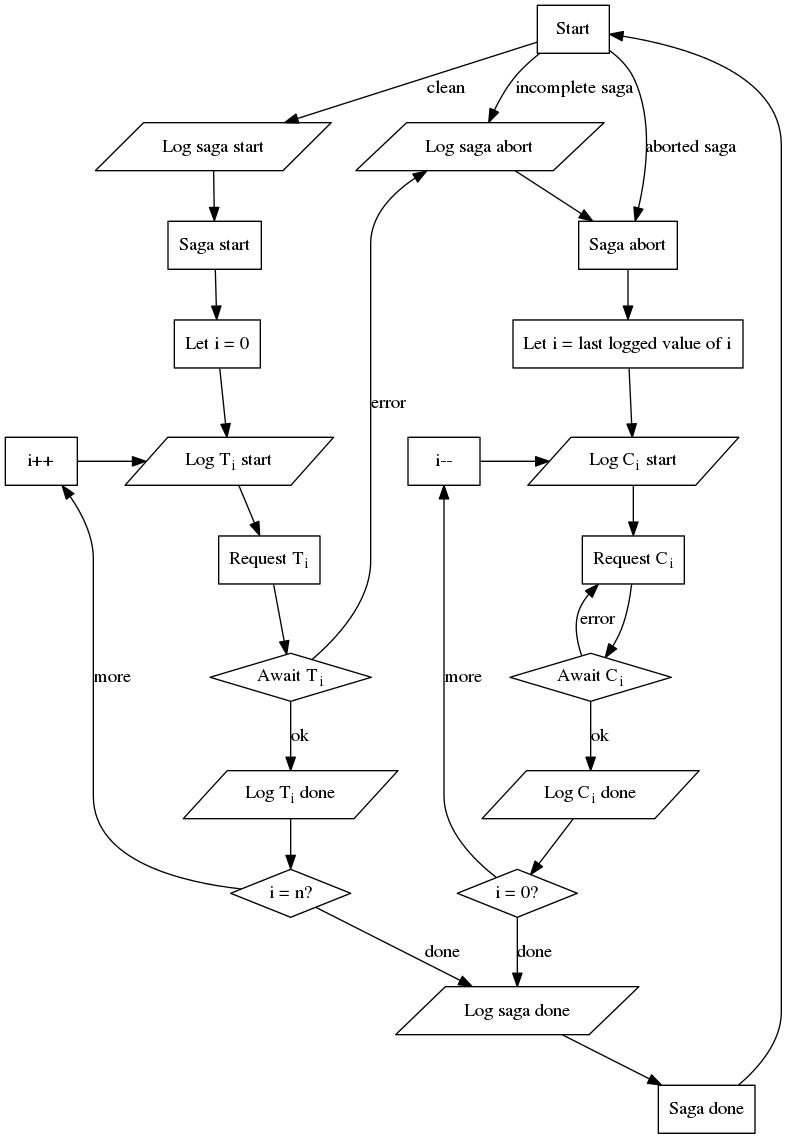
\includegraphics[width=\linewidth]{flow}




\section{Both Rollback and Roll-forward}

\begin{lemma}[]
\label{t_contiguous}
If $T_i$ is received by a TEC, then $T_0, T_1, ... T_{i-1}$ have already been
acknowledged by a TEC, where $0 < i \le n$.
\end{lemma}

\begin{proof}

In order for $T_i$ to be received by a TEC, it must have been requested by an
SEC. In a roll-forward SEC, this could be a retry of a failed attempt to
execute $T_i$, but regardless of whether the SEC is roll-back or roll-forward,
entering that part of the algorithm requires the SEC to journal its intent to
start $T_i$.

There are only two paths to that journaling operation. The first case, $i = 0$,
falls outside our constraint $0 < i \le n$. Therefore the SEC \textit{must}
have taken the other path: incrementing $i$ before beginning a new transaction.

That path depends on $i - 1 \ne n$ being false, which holds since we are
considering $i \le n$. That in turn depends on journaling $T_{i-1}$'s
completion, which depends on a successful response from a TEC for $T_{i-1}$.
Therefore some TEC acknowledged $T_i$. That in turn requires that TEC to have
received $T_i$.

So, the receipt of $T_i$ implies both the receipt and acknowledgement of
$T_{i-1}$. By induction, receiving $T_i$ implies \textit{all} transactions
$T_0, T_1, ... T_{i-1}$ have been acknowledged.

\end{proof}


\begin{corollary}
\label{t_zero_first}
The first transaction to be received and acknowledged is $T_0$.
\end{corollary}

\begin{proof}

Assume the first transaction to be processed is not $T_0$, but rather, some
$T_i \mid 0 < i \le n$. By \ref{t_contiguous}, $T_{i-1}$ must have been
received and acknowledged by a TEC already. $T_i$ is therefore \textit{not} the
first transaction: a contradiction.

\end{proof}


\begin{lemma}
\label{c_prior_ts}
If $C_i$ is received by a TEC, then $T_{i - 1}$ must have been acknowledged by
some TEC, where $0 < i \le n$.
\end{lemma}

\begin{proof}

Receipt of $C_i$ by a TEC implies the request of $C_i$ by some SEC. An SEC can
only request $C_i$ if it logs its intent to start $C_i$, which can occur by two
paths: either the completion of $C_{i+1}$, or by the initialization of $i$ to
its last logged value. Both branches imply the SEC read $i$, or some higher
value, from storage.

$i$ is only incremented by an SEC which has successfully completed $T_{i-1}$.
Since $i$ is nonzero, it was incremented, and $T_{i-1}$ was acknowledged by
some TEC.

\end{proof}


\begin{lemma}
\label{c_maybe_t}
If $C_i$ is requested, $T_i$ may or may not have been requested.
\end{lemma}

\begin{proof}

We know from \ref{c_prior_ts} that $C_i$ implies the acknowledgement of all
$T_j$ where $0 \le j < i$. But what of that final transaction, $T_i$? Can we
guarantee its completion?

The answer is no. All that is necessary for $C_i$ to occur is for an SEC to
write $T_i$'s start. If the SEC crashes just after journaling, it will never
request $T_i$. If it does not crash, $T_i$ will be requested.

\end{proof}


\begin{lemma}
\label{max_c_later_ts}
If $C_i$ is the highest compensating transaction requested, no $T_j$ will ever
have been requested, for all $i < j$.
\end{lemma}

\begin{proof}

Assume some $T_j$ subsequent to $T_i$ \textit{is} requested. Then some SEC must
have written $j$ to storage prior to that request. In order to reach $C_i$, an SEC must have received acknowledgement for $C_j$ first, which implies $C_i$ is not the highest compensating transaction requested: a contradiction.

\end{proof}

\begin{lemma}
\label{max_t_later_cs}
If $T_i$ is the highest transaction requested, no $C_j$ will ever have been
requested, for all $i + 1 < j$.
\end{lemma}

\begin{proof}

Assume some $C_j$ \textit{is} eventually requested. Then some SEC must have written $j$ to disk, which implies $T_{j-1}$ was acknowledged. Since $T_{j-1}$ was requested, and $i < j - 1$, $T_i$ cannot have been the highest transaction requested: a contradiction.

\end{proof}


\begin{lemma}
\label{success_all_ts}
If a saga completes successfully, every transaction $T_i$ will have been
acknowledged at least once, for $0 \le i \le n$.
\end{lemma}

\begin{proof}

A saga can complete successfully iff the highest transaction $T_n$ has been
acknowledged. By \ref{t_contiguous}, every $T_i$ must \textit{also} have
completed, where $0 \le i < n$.

\end{proof}


\begin{lemma}
\label{abort_corresponding_cs}
If a saga completes the abort process, and $T_i$ was received by a TEC, $C_i$
was also acknowledged by a TEC.
\end{lemma}

\begin{proof}

Let $C_{m}$ be the highest compensating transaction acknowledged. Assume $C_i$
was not received: $m < i$. By \ref{max_c_later_ts}, no transaction $T_i$ with
$m < i$ can ever occur, so $i \le m$---which contradicts $m < i$. $C_i$ must
have been acknowledged.

\end{proof}


\begin{theorem}
\label{all_ts_or_corresponding_cs}
Once a saga is complete, either every transaction $T_i$ will have been acknowledged at least once; or, for every transaction $T_i$ received by a TEC, $C_i$ is also acknowledged by a TEC.
\end{theorem}

\begin{proof}

Sagas may only complete by successful termination or by being aborted. If
successful, \ref{success_all_ts} ensures every $T_i$ occurs. If the saga
aborts, \ref{abort_corresponding_cs} ensures the receipt of $T_i$ implies the
receipt of $C_i$.

\section{Rollback}

\begin{lemma}
\label{t_at_most_once}
Transactions are requested and received at most once.
\end{lemma}

\begin{proof}

In order for an SEC to request a transaction $T_i$, it has to record its intent
to execute $T_i$ in shared SEC storage. Since that storage is linearizable, any
other SEC recording an intent to execute $T_i$ would be visible to the
requesting SEC.

\begin{description}
  \item[Case 1] Another SEC has already recorded its intent to request $T_i$.
The given SEC chooses to crash instead of requesting $T_i$.
  \item[Case 2] No other SEC has recorded its intent to request $T_i$. The
given SEC requests $T_i$ once.
\end{description}

In both cases, $T_i$ is requested at most once, across all SECs, depending on
whether or not the successfully-recording SEC crashes before making its
request.

Because the network does not duplicate requests, the number of times $T_i$ can
arrive at a TEC is less than or equal to the number of requests any SEC makes
for $T_i$. Since that number is at most one, $T_i$ is received at most once.

\end{proof}


\begin{lemma}
\label{t_sequential}
Transactions are seen by TECs in sequential order: $T_0, T_1, \ldots, T_j$,
where $0 \le j \le n$.
\end{lemma}

\begin{proof}

Consider a sequential history $S = (T_0, ..., T_i)$ followed by $T_j$. Is $(T_0,
... T_i, T_j)$ sequential? We must show $i + 1 = j$.

\begin{description}
  \item[Case 1] Assume $j \le i$. Then $T_j$ is a duplicate of some transaction
already in $S$, which violates \ref{t_at_most_once}: a contradiction.
  \item[Case 2] Assume $i + 1 < j$. By \ref{t_contiguous}, $T_{i + 1}$ must
appear before $T_j$---but $S$ cannot contain $T_{i+1}$, since it only ranges
from $0$ to $T_i$.
  \item[Case 3] Assume $i < j \le i + 1$. Then $i + 1 = j$.
\end{description}

Since cases 1 and 2 are impossible, \textit{any} history comprised of a
transaction following a sequential history of at least one element must be
sequential as well.

Now, consider histories of one element or fewer:

\begin{description}
  \item[Case 1] No transactions occur. The history is trivially sequential.
  \item[Case 2] Exactly one transaction occurs. By \ref{t_zero_first}, that
transaction must be $T_0$. This history is trivially sequential.
\end{description}

So any history of one element or fewer is sequential, and any transaction
\textit{appended} to that history will also form a sequential history, and so
on. By induction, all transactions in a rollback saga system occur
sequentially.

\end{proof}

\end{document}
